\documentclass[aspectratio=169,11pt]{beamer}
\usetheme{Madrid}
\usecolortheme{seahorse}
\useinnertheme{rectangles}

\setbeamertemplate{navigation symbols}{}
\setbeamerfont{frametitle}{size=\large,series=\bfseries}
\setbeamerfont{title}{size=\Large,series=\bfseries}

\usepackage{booktabs}
\usepackage{graphicx}
\usepackage[T1]{fontenc}
\usepackage[utf8]{inputenc}
\usepackage{tikz}
\usetikzlibrary{arrows.meta,positioning,calc}

\graphicspath{{../figures/}}

\title[Risk-adjusted stablecoin cost]{The Risk-Adjusted Cost of Stablecoins as Payment Instruments}
\subtitle{An international comparison}
\author[A. Alonso-Robisco]{Andrés Alonso-Robisco}
\institute[BdE]{Banco de España}
\date{\today}

\begin{document}

% =====================================================================
% Slide 1 — Title
% =====================================================================
\begin{frame}[plain]
\titlepage
\end{frame}

% =====================================================================
% Slide 2 — The puzzle
% =====================================================================
\begin{frame}{The puzzle}
\textbf{Stablecoin fees look two orders of magnitude cheaper than incumbent rails.}

\bigskip

\begin{itemize}
  \item US--Mexico retail remittance via correspondent banking: \textbf{$\sim$330 bps} (World Bank, 2025).
  \item Same payment via USDT on Tron: \textbf{$\sim$37 bps}.
\end{itemize}

\smallskip
The headline narrative \,---\, \emph{stablecoins are a payment frontier} \,---\, rests on this gap.

\bigskip

\textbf{But this prices fees, not exposure.} The sender holds a private-issuer liability the standard comparison does not price.
\end{frame}

% =====================================================================
% Slide 3 — The hidden cost: two coupled risks
% =====================================================================
\begin{frame}{The hidden cost: two coupled risks}
A stablecoin promises convertibility at par. The promise can fail in two coupled ways.

\bigskip

\begin{itemize}
  \item \textbf{Counterparty risk.} The issuer's reserve may not be liquid or transparent enough to honour redemption at par.
  \item \textbf{Depeg risk.} The secondary conversion market has finite depth; the realised price slips below par under selling pressure.
\end{itemize}

\bigskip

\textbf{The two reinforce each other.} Issuer stress fuels selling pressure on the secondary market; a deeper depeg signals issuer fragility.

\bigskip

They cannot be priced separately. \,---\, \emph{coordination problem, next slide.}
\end{frame}

% =====================================================================
% Slide 4 — Why a coordination game (Global game intuition)
% =====================================================================
\begin{frame}{Why a coordination game?}
Each holder's redemption depends on what others do; the aggregate run depends on each holder's decision.

\bigskip

\begin{center}
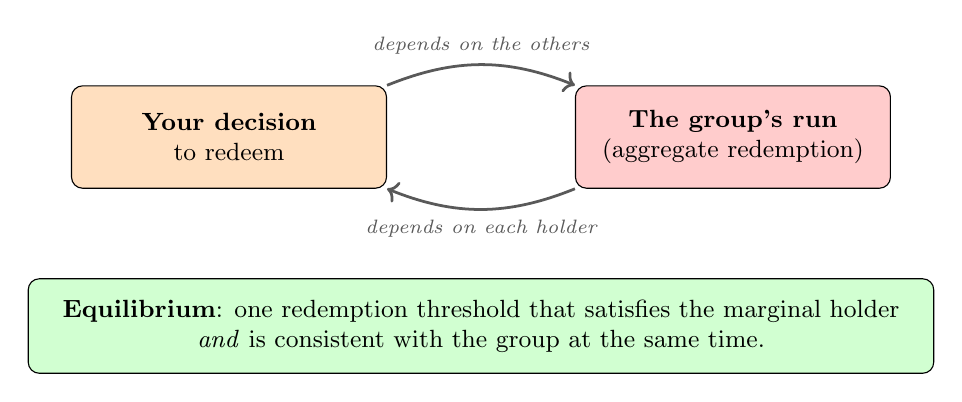
\begin{tikzpicture}[font=\small, every node/.style={align=center}]
  \node[draw, rounded corners, fill=orange!25, minimum width=4.0cm, minimum height=1.3cm] (you) at (-3.2, 0)
    {\textbf{Your decision}\\to redeem};
  \node[draw, rounded corners, fill=red!20, minimum width=4.0cm, minimum height=1.3cm] (group) at (3.2, 0)
    {\textbf{The group's run}\\(aggregate redemption)};

  \draw[->, line width=1pt, gray!70!black]
    (you.north east) to[bend left=22]
    node[above, font=\scriptsize\itshape] {depends on the others} (group.north west);
  \draw[->, line width=1pt, gray!70!black]
    (group.south west) to[bend left=22]
    node[below, font=\scriptsize\itshape] {depends on each holder} (you.south east);

  \node[draw, rounded corners, fill=green!18, minimum width=11.5cm, minimum height=1.2cm] at (0, -2.4)
    {\textbf{Equilibrium}: one redemption threshold that satisfies the marginal holder\\\emph{and} is consistent with the group at the same time.};
\end{tikzpicture}
\end{center}

\medskip

Solved with the \textbf{Morris--Shin (1998)} global game; calibrated separately to \textbf{SVB} (USDC) and \textbf{Terra} (USDT).

\vfill
{\tiny\emph{Assumption}: stablecoin holders earn zero nominal yield, in line with the U.S. GENIUS Act (§16(a), 2025) and EU MiCA (Article 50, 2024) prohibition of interest on payment stablecoins and e-money tokens.}
\end{frame}

% =====================================================================
% Slide 5 — Use cases
% =====================================================================
\begin{frame}{Empirical comparison: three retail corridors}
\textbf{Three corridors chosen to span the policy-relevant space.}

\bigskip

\begin{center}
\renewcommand{\arraystretch}{1.4}
\begin{tabular}{llll}
\toprule
& \textbf{Corridor} & \textbf{Amount} & \textbf{Stablecoin vs incumbent} \\
\midrule
\textbf{UC1} & Brazil domestic retail   & USD 40        & USDT-on-Tron \;\textbf{vs}\; PIX \\
\textbf{UC2} & US--Mexico remittance    & USD 400       & USDT-on-Tron \;\textbf{vs}\; SWIFT / Wise \\
\textbf{UC3} & EU--Brazil cross-border  & USD 1{,}000   & USDC \;\textbf{vs}\; SWIFT / Wise \\
\bottomrule
\end{tabular}
\end{center}

\bigskip

\small
\begin{itemize}
  \item \textbf{UC1} \,---\, public rail (PIX) already operating.
  \item \textbf{UC2} \,---\, canonical retail remittance, no public alternative.
  \item \textbf{UC3} \,---\, cross-border under MiCA + Banco Central do Brasil Resolution 561/2026. \textbf{USDC} as the MiCA-compliant choice.
\end{itemize}
\end{frame}

% =====================================================================
% Slide 6 — Data sources
% =====================================================================
\begin{frame}{Data sources}
\small
\textbf{Calibration (risk premium).}
\begin{itemize}\itemsep1pt
  \item Stablecoin prices: \textbf{CryptoCompare} hourly USDC--USD, USDT--USD.
  \item Stress events: \textbf{SVB} (USDC, March 2023, 96h); \textbf{Terra} (USDT, May 2022, 97h).
  \item Issuer parameters: Circle / Tether-BDO attestations; NYAG and CFTC 2021 settlements.
\end{itemize}

\bigskip

\textbf{Cost comparison.}
\begin{itemize}\itemsep1pt
  \item Incumbent fees: \textbf{World Bank RPW Q3 2025}; SWIFT GPI; Wise / Remitly published rates.
  \item Stablecoin on-chain fees \,---\, \emph{next slide.}
  \item Off-ramp basis: empirical stablecoin--local-currency deviation vs official FX, 6-month window.
  \item Working-capital rates: SOFR (US), ECB MRO (EU), Selic (BR).
\end{itemize}
\end{frame}

% =====================================================================
% Slide 6 — Chain choice assumption
% =====================================================================
\begin{frame}{On-chain fee: which chain do we price?}
\small
\textbf{Stablecoin transfers happen on many chains. Cost varies by two orders of magnitude.}

\medskip
\begin{center}
\renewcommand{\arraystretch}{1.2}
\begin{tabular}{lll}
\toprule
\textbf{Chain} & \textbf{Fee for a USD 1{,}000 transfer} & \textbf{Used in} \\
\midrule
USDT on Tron (post-Aug 2025)            & \,\$0.50--\$2 \,($\sim$5--20 bps)    & UC1, UC2 \\
USDC on Solana / Base / Polygon         & \,\$0.01--\$1 \,($\sim$0.1--10 bps)  & UC3 \\
USDC on Ethereum mainnet                & \,\$5--\$30 \,(50--300 bps; $>$300 in congestion) & \textbf{not used} \\
\bottomrule
\end{tabular}
\end{center}

\medskip
\textbf{UC3 (EU--Brazil):} the flat \textbf{15 bps} on-chain cost embeds these assumptions (low-fee L1/L2 chain).

\medskip
\textbf{Off-ramp basis (Brazil, UC3):} \textbf{21 bps}, the average USDC--BRL deviation against the official USD--BRL FX rate on a 6-month rolling window.
\end{frame}

% =====================================================================
% Slide 7 — Anatomy of the holding risk premium
% =====================================================================
\begin{frame}{Anatomy of the holding risk premium}
\centering
\includegraphics[width=0.78\textwidth]{fig_payment_anatomy_preview.pdf}

\vspace{3mm}
{\footnotesize The total cost of a stablecoin payment is the on-chain fee plus a structural holding-risk premium that decomposes into counterparty, baseline-regime depeg, and stress-regime depeg legs.}
\end{frame}

% =====================================================================
% Slide 5 — Per-asset results
% =====================================================================
\begin{frame}{Same machinery, two inverted profiles}
\begin{center}
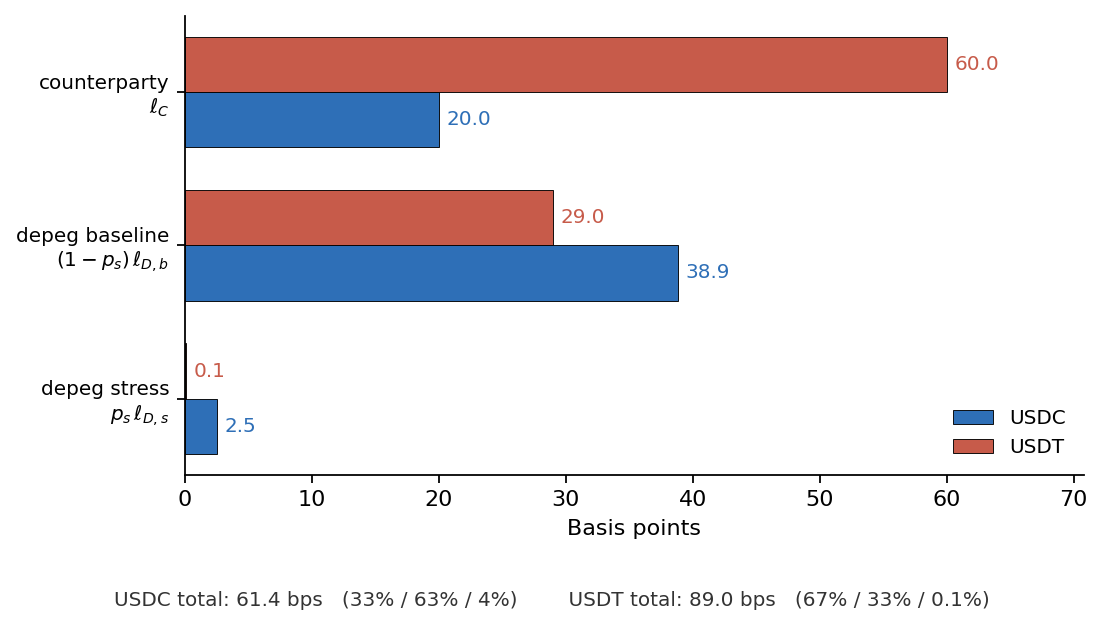
\includegraphics[width=0.86\textwidth]{fig_risk_decomposition.pdf}
\end{center}

\medskip

\begin{itemize}
  \item \textbf{USDC} \,---\, 61 bps, \textbf{depeg-dominant} (63\% / 33\%).
  \item \textbf{USDT} \,---\, 89 bps, \textbf{counterparty-dominant} (67\% / 33\%).
\end{itemize}

\bigskip

Same machinery, two different binding constraints: secondary-market depth (USDC) vs reserve composition (USDT).
\end{frame}

% =====================================================================
% Slide 10 — Bottom line: total cost by use case
% =====================================================================
\begin{frame}{Bottom line: total cost by use case}
\centering
\renewcommand{\arraystretch}{1.3}
\footnotesize
\resizebox{\textwidth}{!}{%
\begin{tabular}{llrrl}
\toprule
\textbf{Use case} & \textbf{Stablecoin path} & \textbf{Total (bps)} & \textbf{Best alternative (bps)} & \textbf{Net outcome} \\
\midrule
UC1 \,---\, BR retail (USD 40)        & USDT-on-Tron & 485 & PIX (0)     & PIX wins by 485 \\
UC2 \,---\, US--MX (USD 400)          & USDT-on-Tron & 139 & Wise (251)  & USDT wins by 112 \\
UC3 \,---\, EU--BR (USD 1{,}000)      & USDC         & 97  & Wise (205)  & USDC wins by 108 \\
\bottomrule
\end{tabular}%
}

\bigskip

\textbf{Three regimes of payments innovation.}
\begin{itemize}\small\itemsep1pt
  \item Where a public instant-payment rail exists today (UC1, PIX), the stablecoin is dominated.
  \item Where it does not (UC2, UC3), the stablecoin wins net of its structural risk premium.
  \item Once an upgraded public cross-border rail goes live (BIS Nexus, mid-2027 on UC2/UC3 corridors), the stablecoin advantage is absorbed.
\end{itemize}
\end{frame}

% =====================================================================
% Slide 7 — Policy takeaways
% =====================================================================
\begin{frame}{Policy takeaways}
\begin{enumerate}
  \item \textbf{Build versus license.}\\
  Building upgraded public cross-border infrastructure (Nexus, Agorá) has a first-order effect on stablecoin substitution.

  \medskip
  \item \textbf{The risk premium is structural, not operational.}\\
  Faster bridges, cheaper gas, or better wallets do not reduce it. It reflects the substance of holding a private-issuer liability.

  \medskip
  \item \textbf{Per-issuer supervision.}\\
  USDC's binding constraint is secondary-market depth; USDT's is reserve composition. The same coordination logic returns two different supervisory priorities.
\end{enumerate}

\vfill
\centering
\small\emph{Thank you. Questions welcome.}
\end{frame}

\end{document}
